\chapter{Background}
\label{chap:background}

\section{Mathematical Foundation}
The following discussion of the homomorphic encryption schemes requires some mathematical background that
will (at least partially) be introduced here.

Let $\N$ denote the natural numbers without $0$, i.e. $\N = \{n \in \Z \,|\, n > 0\}$.
For a probability distribution $\chi$ over a set $R$, let sampling a value $x \in R$ from the probability distribution be denoted by $x \leftarrow \chi$.
For $a \in \R$ a real number, denote rounding down (floor) $a$ by $\lfloor a \rfloor \in \Z$,
rounding up (ceil) by $\lceil a \rceil \in \Z$ and rounding to the nearest integer by
$\lfloor a \rceil \in \Z$.

\begin{definition}{Ring}{ring}
  A tuple $(R, +, \cdot)$ consisting of a set $R$, an addition operation $+$ and a multiplication operation $\cdot$
  is referred to as a ring, given that it satisfies the following \textit{ring axioms}:
  \begin{itemize}
    \item Addition is closed: $a + b \in R \quad\forall a, b \in R$.
    \item Addition is commutative: $a + b = b + a \quad\forall a, b \in R$.
    \item Addition is associative: $(a + b) + c = a + (b + c) \quad\forall a, b, c \in R$.
    \item There exists an element $0 \in R$ such that $a + 0 = a \quad\forall a \in R$.
    \item An additive inverse $-a$ of each element $a$ in $R$ exists, such that $a + (-a) = 0$.
    \item Multiplication is associative: $(a \cdot b) \cdot c = a \cdot (b \cdot c) \quad\forall a, b, c \in R$.
    \item Multiplication is closed: $a \cdot b \in R \quad\forall a, b \in R$.
    \item There exists an element $1 \in R$, referred to as the identity element, or multiplicative identity of $R$,
          such that $a \cdot 1 = a \quad\forall a \in R$.
    \item Multiplication $\cdot$ is distributive w.r.t. addition $+$, \\
          i.e. $a \cdot (b+c) = (a \cdot b) + (a \cdot c) \quad\forall a, b, c \in R$ from the left and \\
          i.e. $(b+c) \cdot a = (b \cdot a) + (c \cdot a) \quad\forall a, b, c \in R$ from the right.
  \end{itemize}
  Where the first 5 properties can be summarised as $(R, +)$ forming an Abelian group.
  If multiplication is additionally commutative, we refer to the ring as commutative:
  \begin{itemize}
    \item Multiplication is commutative: $a \cdot b = b \cdot a \quad\forall a, b \in R$.
  \end{itemize}
\end{definition}
Acting as a logical extension of a group, a ring can be considered the intermediary step towards a field
(which also defines subtraction and division).
An example of a ring would be the integers modulo $t$: $\Z / t \Z$, sometimes also denoted as $\Z_t$.

\begin{definition}{Quotient Group / Ring}{quotient-group}
  A quotient group $(G / N, +)$ (pronounced '$G$ mod $N$') over the original group $G$ and a normal subgroup $N$ of $G$
  with a standard element operation $+$ can be defined using the left cosets
  $$g+N := \{g+n \,|\, n \in N\} \subseteq G$$ of $N$ in $G$.
  The corresponding set $G / N$ is defined as
  $$G / N := \{g + N \,|\, g \in G\}$$
  whereas the standard operation $+: G/N \times G/N \mapsto G/N$
  can be extended from the original group $G$ as follows:
  $$(g+N) + (h+N) := (g+h)N$$
\end{definition}

The quotient set $G / N$ can therefore be identified as the set of all possible left cosets $g + N$ that in union reconstruct the original group $G$.

\begin{definition}{Ring of Integers Modulo $t$: $\Z / t \Z$}{integers-modulo-t}
  Using equivalence classes $\overline{x}_t$ modulo $t$ referred to as congruence classes,
  define the commutative quotient ring of integers modulo $t$ as $(\Z / t \Z, +, \cdot)$ with
  two operations $+$ and $\cdot$ and
  $$\Z / t \Z = \{\overline{x}_t \,|\, x \in \Z, 0 \leq x < t\}$$
  where $t \Z \triangleleft \Z$ denotes the $t$\textsuperscript{th} multiplicative coset\footnote{
    from the left and from the right, therefore $t \Z$ is called a normal subgroup of $\Z$
  } of the integers and
  $$\overline{x}_t = \{y \equiv x \mod t \,|\, y \in \Z\}$$
  is the set of all multiples of $t$ with remainder $x$.
  Note that many operations that resulting groups, rings or fields are commonly equipped with,
  such as addition or multiplication, propagate to an equivalent definition in the ring of integers modulo $t$
  by considering their result as a congruence class instead of it, which in turn is again an element of $\Z / t \Z$.
\end{definition}

\begin{definition}{Polynomial Ring over $\Z$}{poly-ring}
  On the set of all complex-valued polynomials with integer coefficients (a function space)
  $$\Z[X] = \big\{p: \C \mapsto \C \,, p(X) = \sum_{k=0}^\infty a_k X^k, a_k \in \Z \;\forall k \geq 0\big\},$$
  we can define a commutative ring $(\Z[X], +, \cdot)$ equipped with the
  standard addition $+$ and multiplication $\cdot$ operations (as an extension over the field $\C$)
  of polynomials.
\end{definition}

To further elaborate on the polynomial ring operations:
\begin{itemize}
  \item In their coefficient representations $\vec{p} = (p_j)_{j\in\N} = (p_0, p_1, p_2, ...)$ (which are sequences) and $\vec{q} = (q_j)_{j\in\N} = (q_0, q_1, q_2, ...)$,
        an addition of two polynomials $p, q \in \Z[X]$ is equivalent to the element-wise addition of their coefficient sequences
        \begin{align*}
          (p + q)(X) & = \sum_{k=0}^\infty p_k X^k + \sum_{k=0}^\infty q_k X^k = \sum_{k=0}^\infty (p_k + q_k) X^k \\
                     & = \langle (\vec{p} + \vec{q}), \{X^0, X^1, X^2, ...\}^T \rangle
        \end{align*}
        which indeed satisfies the additive \hyperref[def:ring]{ring axioms}
        due to the existing structure of the underlying field $\C$.
  \item The multiplication operation can be defined using a discrete convolution of the coefficient vectors
        $$r(X) = (p \cdot q)(X) = (\sum_{k=0}^\infty p_k X^k) \cdot (\sum_{l=0}^\infty q_l X^l)
          = \sum_{k=0}^\infty \sum_{l=0}^\infty p_k q_l X^{k+l}
          = \sum_{k=0}^\infty r_k X^k$$
        with the arising coefficients $(r_k)_{k\in\N}$ determined by the discrete convolution
        $$r_k = \sum_{l=0}^k p_l q_{k-l} \;\Leftrightarrow\; \vec{r} = \vec{p} * \vec{q}$$
        in this context also referred to as the \name{Cauchy}-product. Therefore,
        $$(p \cdot q)(X) = \langle (\vec{p} * \vec{q}), \{X^0, X^1, X^2, ...\}^T \rangle.$$
        Again, this generally applicable approach satisfies the multiplicative \hyperref[def:ring]{ring axioms}
        and even satisfies commutativity due to the existing structure of the underlying field $\C$
        and the symmetry of convolutions.
\end{itemize}

Where $\langle \cdot, \cdot \rangle$ denotes the dot (scalar) product between two vectors.

Polynomials with degree $\geq 1$ over the complex numbers can always be factorised using their roots due to the fundamental theorem of algebra.
Polynomials over the integers however, cannot always be factorised further, yielding the definition of an irreducible polynomial.

\begin{definition}{Irreducible Polynomials}{irreducible-polys}
  A polynomial is called irreducible \glstext{iff} it cannot be written as a product of other polynomials
  \textsl{while staying in the same coefficient space}.
\end{definition}

\subsection{Cyclotomic Polynomials}
Due to their interesting structure and efficient computability, in the schemes introduced in the following chapter, certain polynomials (\autoref{corollary:bounded-polynomials-mod-q}) are chosen as representations of plaintexts and ciphertexts.
An important concept is that of cyclotomic ('circle-cutting') polynomials, which we will discuss in a bit more detail here.

An important polynomial is $$p: \C \mapsto \C, \; p(x) = x^n - 1$$.
Its roots, found by solving $p(x) = 0$ for $x$, yielding $x^n = 1 \leftrightarrow x_k = \sqrt[n]{1}$ are referred to as the $n$\textsuperscript{th} roots of unity, of which there are multiple for each $n \in \N$.

\begin{lemma}{The $n$\textsuperscript{th} roots of unity}{nth-roots-of-unity}
  For some integer $n \in \N$, the $n$ complex roots $x_1, x_2, ..., x_n \in \C$ of unity
  can be found as $$x_k = e^{2\pi i \frac{k}{n}} \quad k \in \{1, 2, ..., n\}$$
  with $i$ the imaginary unit.
  Using \name{Euler}'s identity, their real and imaginary components can be explicitly found as
  $x_k = \cos(2\pi \frac{k}{n}) + i \sin(2\pi \frac{k}{n})$.

  An $n$\textsuperscript{th} root of unity $y$ is referred to as \textit{primitive}, \glstext{iff}
  there exists no $m < n$ for which that root $y$ is also an $m$\textsuperscript{th} root of unity, i.e. $y^m \neq 1$.
  An equivalent indicator is when $\gcd(m, n) = 1$.
\end{lemma}
Due to the fact that for any $k, l \in \Z$, their product $x_k \cdot x_l$ is also a root of unity, and
$x_{k+jn} = x_k \; \forall j \in \Z$, they clearly comprise a cyclic Abelian group over the complex numbers
$\C$ under multiplication with (for instance) the first root $x_1 = e^{2\pi i \frac{1}{n}}$ as its generator.

\begin{definition}{Cyclotomic Polynomial}{cyclotomic-poly}
  Given the $n$\textsuperscript{th} roots of unity $\{x_k\}$, we can define the $n$\textsuperscript{th}
  cyclotomic polynomial $\Phi_n \in \Z[X]$ as the product over all primitive roots of unity
  $$\Phi_n(x) = \prod_{\stackrel{k=1}{x_k \mathrm{primitive}}}^{n} (x - x_k)$$
  It is unique for each given $n \in \N$.
\end{definition}
The number of primitive roots of unity is given by $\varphi(n)$, denoting Euler's totient function which counts the
natural numbers $m$ less than $n$ who do not share a common divisor $\neq 1$, i.e. $\gcd(m, n) = 1$.
$\varphi(n)$ therefore also counts the number of primitive roots of unity for $n$,
consequently also yielding the degree of the $n$\textsuperscript{th} cyclotomic polynomial.

\begin{remark}{Irreducibility of Cyclotomic Polynomials}{cyclotomic-irreducibility}
  Cyclotomic polynomials are always irreducible.
\end{remark}
The proof for \autoref{remark:cyclotomic-irreducibility} is quite cumbersome, but can be found in \cite{2002-serge-algebra}.

\begin{theorem}{$2^k$\textsuperscript{th} cyclotomic polynomial}{power-of-2-cyclo-poly}
  The $n$\textsuperscript{th} cyclotomic polynomial, where $n = 2^k$ ($k \in \N$) is a power of $2$,
  can be identified as
  $$\Phi_{n}(x) = x^{n/2} + 1\,.$$
  Its degree is $n/2$, consistent with $\varphi(2^k) = 2^{k-1} \; \forall k \in \N$.
\end{theorem}
Find a short but illustrative proof of \autoref{thm:power-of-2-cyclo-poly} in the \hyperref[chap:appendix]{Appendix}.

\begin{definition}{Ring of Polynomials of highest degree $N-1$}{bounded-polynomials}
  One can construct the quotient ring $(R, +, \cdot)$ as
  $$R = \Z[X] / (X^N + 1)$$
  where $(X^N + 1)$ denotes the set of all polynomial multiples of the polynomial $p \in \Z[X], p(x) = x^N + 1$, so
  $$(X^N+1) = \{q: \C \mapsto \C,\; q(x) = r(x) \cdot (x^N+1) \;|\; r \in \Z[X]\}$$
  The elements of $R$ are then polynomials with integer coefficients of maximum degree $N-1$.
\end{definition}

If $N$ is a power of $2$, according to \autoref{thm:power-of-2-cyclo-poly},
$R$ is the set of integer-coefficient polynomials reduced modulo $\Phi_d(X)$
the $d$\textsuperscript{th} cyclotomic polynomial with $N = \varphi(d) = \frac{d}{2}$.
$$R = \Z[X] / \Phi_d(X) = \Z[X] / (X^N + 1)\,.$$
Since every cyclotomic polynomial is irreducible, this is a unique representation of $R$
without any further possible simplifications.

\begin{corollary}{Polynomial Ring modulo $q$}{bounded-polynomials-mod-q}
  Further modifying $R = \Z[X] / (X^N+1)$ to only take coefficients mod $q$, we obtain two equivalent definitions
  for the same ring:
  $$R_q = R/qR = (\Z/q\Z)[X] / (X^N+1)$$
  which contains polynomials with integer coefficients modulo $q$ of degree $N-1$.
  Explicitly stated, the set can be written as:
  $$R/qR = \{p: \C \mapsto \C,\; p(x) = \sum_{k=0}^{N-1} a_k x^k \;|\; a_k \in \Z/q\Z\}$$
\end{corollary}

\subsection{Lattice Cryptography}
To illustrate the connection of these problems to lattices, we take a closer look at them before considering further details of LWE.
Most notably, lattice problems are conjectured to be secure against quantum computers \parencite{2018-lattice-problems}.

\newcommand{\lat}{\mathcal{L}}
\begin{definition}{Lattice}{lattice}
  A lattice $(\lat, +, \cdot)$ is a vector field over the integers $(\Z, +, \cdot)$, defined using a set of $n$ basis vectors $\vec{b_1}, \vec{b_2}, ..., \vec{b_n} \in \R^n$, that can be introduced as a set
  $$\lat = \bigg\{\sum_{i=1}^m c_i \vec{b}_i \,|\, c \in \Z\bigg\} \subseteq \R^n$$
  equipped with at least vector addition $+: \lat \times \lat \mapsto \lat$ and scalar multiplication $\cdot: \Z \times \lat \mapsto \lat$.
  As an extension of $\R^n$, the Euclidean norm $||\cdot||$ is also defined and the standard Euclidean metric $d: \lat \times \lat \mapsto \R$, yielding a metric space $(\lat, d)$, can be obtained by the norm of a vector difference, denoted $||(\cdot) - (\cdot)||$.
\end{definition}

Its \textit{minimum distance} $\lambda_{min}$ is defined as the smallest Euclidean distance between two points $\vec{p_1}$ and $\vec{p_2} \in \lat$
$$\lambda_{min} = \min_{\vec{p_1}, \vec{p_2} \in \lat} d(\vec{p_1}, \vec{p_2}) =
  \min_{\vec{p_1}, \vec{p_2} \in \lat} ||\vec{p_1} - \vec{p_2}|| \,,$$
which can be equivalently thought of as the minimal length of any non-zero vector in the lattice $\lat$, because of $\vec{0}$ always being an element of the lattice which can be chosen as $\vec{p_1}$ and the translational symmetry between fundamental lattice volumes (or regions).

\begin{definition}{Shortest Vector Problem (SVP)}{svp}
  Given a lattice $\lat$ constructed from $n$ basis vectors, find the shortest non-zero lattice vector $\vec{x} \in \lat \backslash \{\vec{0}\}$, i.e. find $\vec{x}$ such that $||\vec{x}|| = \lambda_{min}$ \parencite{2016-decade-of-lattice}.
\end{definition}

\begin{definition}{Decisional Approximate SVP (GapSVP)}{gap-svp}
  Given a lattice $\lat$ and some pre-defined function $\gamma: \N \mapsto \R$ depending on the lattice dimension $n$ (constant for a given $\lat$) with $\gamma(n) \geq 1$, the decisional approximate shortest vector problem is distinguishing between $\lambda_{min} \leq 1$ and $\lambda_{min} > \gamma(n)$.
  For other cases, it is up to the algorithm what to return.
\end{definition}

\begin{definition}{Short Integer Solution (SIS) Problem}{sis}
  For $m$ given vectors $(\vec{a}_i)_{0 < i \leq m} \in (\Z / q\Z)^n$ that comprise the columns of a matrix
  $A \in (\Z / q\Z)^{n \times n}$ and an upper bound $\beta$, find
  a solution vector $\vec{z} \in \Z^n \backslash \{\vec{0}\}$ such that
  $$A \vec{z} = \vec{0} \quad \mathrm{with} \quad ||\vec{z}|| \leq \beta\,.$$
\end{definition}

Note that without the last requirement, the SIS problem can be easily solved through Gaussian elimination or similar algorithms, however they rarely yield a short (or \textit{the} shortest) solution.
It can be shown that solving SIS is at least as hard as solving GapSVP with appropriate parameters \parencite{1996-hard-lattice-problems}.

Using the above problems, multiple cryptographic primitives can be constructed due to the proven hardness that also propagates to quantum computers.
Examples include collision resistant hash functions, signatures, pseudorandom functions or even Regev's public-key cryptosystem \parencite{2016-decade-of-lattice}.

\usetikzlibrary{calc}
\begin{figure}
  \centering
  \begin{tikzpicture}
    \coordinate (Origin)   at (0,0);
    \coordinate (XAxisMin) at (-3,0);
    \coordinate (XAxisMax) at (5,0);
    \coordinate (YAxisMin) at (0,-2);
    \coordinate (YAxisMax) at (0,5);
    \draw [thin, gray, -latex] (XAxisMin) -- (XAxisMax);
    \draw [thin, gray, -latex] (YAxisMin) -- (YAxisMax);

    \clip (-4,-3) rectangle (5.5, 5.5);
    \pgftransformcm{1}{0.3}{0.7}{1}{\pgfpoint{0cm}{0cm}}
    \coordinate (Bone) at (0,2);
    \coordinate (Btwo) at (2,-2);
    \draw[style=help lines,dashed] (-14,-14) grid[step=2cm] (14,14);
    \foreach \x in {-7,-6,...,7}{
        \foreach \y in {-7,-6,...,7}{
            \node[draw,circle,inner sep=2pt,fill] at (2*\x,2*\y) {};
          }
      }
    \draw [ultra thick,-latex,themecolor] (Origin)
    -- (Bone) node [above left] {$\vec{b}_1$};
    \draw [ultra thick,-latex,themecolor] (Origin)
    -- (Btwo) node [below right] {$\vec{b}_2$};
  \end{tikzpicture}
  \caption{Illustration of a standard lattice $\lat$ over the integers $\Z$
    with two basis vectors $\vec{b}_1$ and $\vec{b}_2$, c.f. \autoref{def:lattice}.
    The shortest vector problem in this case is solved by $\vec{x} = 0 \vec{b}_1 \pm 1 \vec{b}_2$.}
  \label{fig:lattice}
\end{figure}


\subsection{Learning with Errors (LWE)}
\label{subsec:lwe}
Next, we would like to consider \Gls{lwe}, a computing problem that is believed to be sufficiently hard to be used in cryptography and, most notably, is not yet solvable in linear time by a quantum algorithm (c.f. \autoref{sec:post-quantum-sec}).
Its hardness assumptions were first formally proven by \citeauthor{2005-lwe-original}, for which he received the 2018 Gödel price.

\begin{definition}{LWE-Distribution $A_{\vec{s}, \chi_{error}}$}{lwe-dist}
  Given a prime $p \in \N$ and $n \in \N$, we choose some secret $\vec{s} \in (\Z / p \Z)^n$.
  In order to sample a value from the LWE distribution $A_{\vec{s}, \chi_{error}}$:
  \begin{itemize}
    \item Draw a random vector $a \in (\Z/p\Z)^n$ from the multivariate uniform distribution
          with its domain in the integers up to $p$.
    \item Given another probability distribution $\chi_{error}$ over the integers modulo $p$,
          sample a scalar 'error term' $\mu \in \Z / p \Z$ from it.
    \item Set $b = \vec{s} \cdot \vec{a} + \mu$, with $\cdot$ denoting the standard vector product.
    \item Output the pair $(\vec{a}, b) \in (\Z / p \Z)^n \times (\Z / p \Z)$.
  \end{itemize}
\end{definition}

The general approach useful to cryptography is to sample an element from the LWE-distribution and construct
two problems out of it, \textit{search}-LWE and \textit{decision}-LWE.

\begin{definition}{LWE-Problem - Search Version}{lwe-search-problem}
  Given $m$ independent samples $(\vec{a}_i, b_i)_{0 < i \leq m}$ from $A_{\vec{s}, \chi_{error}}$, find the secret $\vec{s}$.
\end{definition}
\begin{definition}{LWE-Problem - Decision Version}{lwe-decision-problem}
  Given $m$ samples $(\vec{a}_i, b_i)_{0 < i \leq m}$, distinguish (with non-negligible advantage) whether they were drawn from $A_{\vec{s}, \chi_{error}}$ or from the uniform distribution $u$ over $(\Z / p \Z)^n \times (\Z / p \Z)$.
\end{definition}

In their above definitions, \citeauthor{2005-lwe-original} showed that the two problems are equivalent.

\begin{theorem}{Hardness of LWE}{lwe-hardness}
  If there exists an efficient algorithm that solves either search-LWE or decision-LWE then there exists an efficient quantum algorithm that approximates the decision version of the shortest vector problem (GapSVP) in the worst case \parencite{2010-lwe-survey}.
\end{theorem}

He also provided a construction of a public-key cryptosystem based on them, i.e. an asymmetric cryptographic system for at least two parties that includes a public and corresponding private key.

Public-key cryptosystems are fundamentally different from symmetric systems, which only require one single key for encryption and decryption at the same time, known by all involved parties.
Often times, public-key schemes (rather slow) are used to exchange keys for subsequent symmetric encryption (rather fast) of large plaintexts, for instance in the \gls{tls} protocol \parencite{rfc8446}.

\subsection{Learning with Errors on Rings (RLWE)}
\Gls{rlwe}
\cite{2010-rlwe-original}
% TODO: how to get from LWE to RLWE

Similar to \autoref{def:lwe-dist}, the Ring-LWE distribution can be derived as follows:

\begin{corollary}{RLWE-Distribution $B_{\vec{s}, \chi_{error}}$}{rlwe-dist}
  Given a quotient \hyperref[def:ring]{ring} $(R/qR, +, \cdot)$, we choose some secret $s \in R/qR$.
  In order to sample a value from the RLWE distribution $B_{s, \chi_{error}}$:
  \begin{itemize}
    \item Uniformly randomly draw an element $a \in R/qR$
    \item Given another probability distribution $\chi_{error}$ over the ring elements,
          sample an 'error term' $\mu \in R/qR$ from it.
    \item Set $b = s \cdot a + \mu$, with $\cdot$ denoting the ring multiplication operation.
    \item Output the pair $(a, b) \in R/qR \times R/qR$.
  \end{itemize}
\end{corollary}

In the exact same manner as \hyperref[subsec:lwe]{above}, the search and decision problems can be constructed.

\begin{corollary}{RLWE-Search Problem}{search-rlwe}
  Given $m$ independent samples $(a_i, b_i)_{0 < i \leq m}$ from $B_{s, \chi_{error}}$, find the secret $s$.
\end{corollary}
\begin{corollary}{RLWE-Decision Problem}{decision-rlwe}
  Given $m$ samples $(a_i, b_i)_{0 < i \leq m}$, distinguish (with non-negligible advantage)
  whether they were drawn from $B_{s, \chi_{error}}$ or from the uniform distribution
  $u$ over $R/qR \times R/qR$.
\end{corollary}

\pagebreak
\section{Machine Learning}
Undoubtedly one of the most prevalent concepts in todays computing world, \gls{ml} has shaped how computers think and how we interact with them significantly.
As Shafi \name{Goldwasser} puts it, 'Machine Learning is somewhere in the intersection of Artificial Intelligence, Statistics and Theoretical Computer Science' \parencite{goldwasserTalk2018}.

Within the scope of this thesis, the basics of neural networks and associated learning methods shall be covered, limited to the category of supervised learning problems (as opposed to unsupervised learning problems).
Supervised learning refers to the machine \textit{training} an algorithm to match some input data (features) with corresponding output data (targets), often related to pattern recognition.
The trained algorithm can then be utilised to match fresh input data with a prediction of the targets.

A popular subset of applications to \gls{ml} are classification problems, predominantly image classification, which was not as easily possible before without a human eye due to the lack of computing power.
Classification problems can be formulated quickly, the goal is to computationally categorize input data (for instance, images) into a predefined set of classes (for instance, cats and dogs).
The primary concept behind \acrlong{ml} is not at all new, linear regression was already employed by \name{Gauß} and \name{Legendre} in the early 19\textsuperscript{th} century; the term 'Neural Network' was first used by \name{McCulloch} and \name{Pitts} in 1943.
Much media attention was earned in the 2000-2010 decade when larger image classification problems became feasible with the increasing computational power of modern computers, up until the advent of Deep Learning \parencite{bishop-pattern-recognition-and-ml}.

\subsection{Linear Regression}
Given an input vector $\vec{x} \in \R^n$, the goal of linear regression is to predict the value of a target $t \in \R$, according to some model $M$.

\subsection{Gradient Descent}
\subsection{Multi-Layered Neural Networks}
\begin{figure}[H]
  \centering
  \begin{neuralnetwork}[height=4]
    \newcommand{\x}[2]{$x_#2$}
    \newcommand{\y}[2]{$\hat{y}_#2$}
    \newcommand{\hfirst}[2]{\small $h^{(1)}_#2$}
    \newcommand{\hsecond}[2]{\small $h^{(2)}_#2$}
    \inputlayer[count=3, bias=true, title=Input\\layer, text=\x]
    \hiddenlayer[count=4, bias=false, title=Hidden\\layer 1, text=\hfirst] \linklayers
    \hiddenlayer[count=3, bias=false, title=Hidden\\layer 2, text=\hsecond] \linklayers
    \outputlayer[count=2, title=Output\\layer, text=\y] \linklayers
  \end{neuralnetwork}
  \caption{A neural network}
\end{figure}

To better understand the implications and possibilities of a large neural network, consider the following universal approximation theorem:

\begin{theorem}{Universal Approximation}{universal-approx}
  If the neural network has at least one hidden layer, proper nonlinear activation functions and enough data and hidden units, it can approximate any continuous function $y(x, w): \R^n \mapsto \R$ arbitrarily well on a compact domain \parencite{1989-HornikMultilayerFN}.
\end{theorem}

Matrix -> Activation Function
\begin{itemize}
  \item Matrix Multiplication (Dense Layer)
  \item Convolutional Layer
  \item Sigmoid Activation
  \item Max Pooling
\end{itemize}

% \subsection{The Backpropagation Algorithm}

\section{Post-Quantum Security}
\label{sec:post-quantum-sec}
\begin{figure}[H]
  \centering
  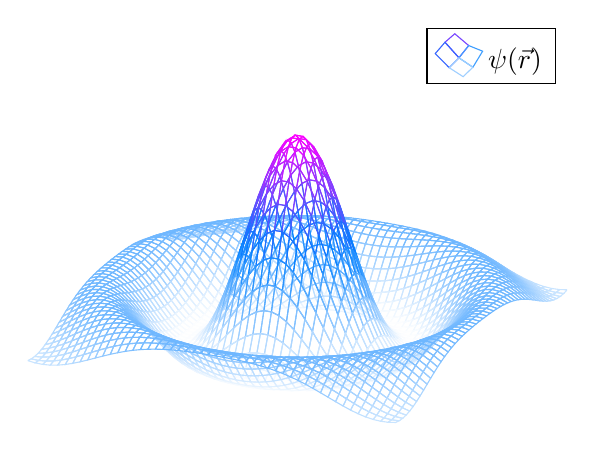
\begin{tikzpicture}
  \begin{axis}[
      % title=Quantum Mechanical Wave Function,
      hide axis,
      colormap/cool
    ]
    \addplot3[
      mesh,
      samples=50,
      domain=-8:8
    ]
    {sin(deg(sqrt(x^2+y^2)))/sqrt(x^2+y^2)};
    \addlegendentry{\(\psi(\vec{r})\)}
  \end{axis}
\end{tikzpicture}

  \caption{Illustration of a wave function $\psi: \R^2 \mapsto \R$ as used in quantum mechanics.}
\end{figure}

\subsection{Shor's Algorithm}

\begin{definition}{NP-Hardness}{np-hard}
  A problem is referred to as \textit{NP-hard} \gls{iff} it is at least as hard as the hardest problems in the complexity class NP (nondeterministic polynomial time). Formally written,
  $$\mathrm{NP} = \bigcup_{k \in \N} \cryptop{NTIME}(n^k)$$
  the union of all decision problems with runtime bounded by $\mathcal{O}(n^k)$.
\end{definition}

\begin{figure}[H]
  \centering
  % This file was created with tikzplotlib v0.10.1.
\begin{tikzpicture}

  \definecolor{darkgray176}{RGB}{176,176,176}
  \definecolor{darkorange25512714}{RGB}{255,127,14}
  \definecolor{lightgray204}{RGB}{204,204,204}
  \definecolor{steelblue31119180}{RGB}{31,119,180}

  \begin{axis}[
      height=0.4\linewidth,
      legend cell align={left},
      legend style={
          fill opacity=0.8,
          draw opacity=1,
          text opacity=1,
          at={(0.03,0.97)},
          anchor=north west,
          draw=lightgray204
        },
      tick align=outside,
      tick pos=left,
      width=0.7\linewidth,
      x grid style={darkgray176},
      xlabel={\(\displaystyle x\)},
      xmin=-5.75, xmax=10.75,
      xtick style={color=black},
      y grid style={darkgray176},
      ylabel={\(\displaystyle y\)},
      ymin=-0.798194220662117, ymax=10.5141997247934,
      ytick style={color=black}
    ]
    \addplot [semithick, steelblue31119180]
    table {%
        -5 0
        0 0
        10 10
      };
    \addlegendentry{$y = \cryptop{relu}(x)$}
    \addplot [semithick, darkorange25512714]
    table {%
        -5 0.590279817581177
        -4.84848499298096 0.478325009346008
        -4.69696950912476 0.374609231948853
        -4.54545450210571 0.27900493144989
        -4.39393949508667 0.191384077072144
        -4.24242401123047 0.111618041992188
        -4.09090900421143 0.0395793914794922
        -3.93939399719238 -0.0248603820800781
        -3.78787875175476 -0.0818290710449219
        -3.63636350631714 -0.131454944610596
        -3.4848484992981 -0.173866033554077
        -3.33333325386047 -0.209190487861633
        -3.18181800842285 -0.237556219100952
        -3.03030300140381 -0.259091377258301
        -2.87878775596619 -0.273924112319946
        -2.72727274894714 -0.282182455062866
        -2.57575750350952 -0.283994436264038
        -2.4242422580719 -0.279488325119019
        -2.27272725105286 -0.268791913986206
        -2.12121200561523 -0.252033472061157
        -1.96969699859619 -0.22934103012085
        -1.81818175315857 -0.200842618942261
        -1.66666650772095 -0.166666269302368
        -1.5151515007019 -0.126940369606018
        -1.36363625526428 -0.0817925930023193
        -1.21212100982666 -0.0313513278961182
        -1.06060600280762 0.0242555141448975
        -0.909090995788574 0.0848997831344604
        -0.757575511932373 0.150453686714172
        -0.60606050491333 0.220788598060608
        -0.454545497894287 0.295776724815369
        -0.151515007019043 0.459200620651245
        0.151515483856201 0.639700412750244
        0.454545497894287 0.836251378059387
        0.757575988769531 1.04782938957214
        1.06060600280762 1.27340888977051
        1.36363649368286 1.51196622848511
        1.66666698455811 1.76247656345367
        1.96969699859619 2.02391457557678
        2.27272748947144 2.29525661468506
        2.57575798034668 2.57547760009766
        3.03030300140381 3.01021504402161
        3.48484897613525 3.45916748046875
        3.93939399719238 3.91887497901917
        4.69696998596191 4.69956493377686
        5.75757598876953 5.79610443115234
        6.21212196350098 6.25772047042847
        6.66666698455811 6.70934343338013
        7.12121200561523 7.14751529693604
        7.42424297332764 7.43045091629028
        7.72727298736572 7.7048454284668
        8.03030300140381 7.96967554092407
        8.33333396911621 8.22391796112061
        8.6363639831543 8.46654510498047
        8.93939399719238 8.69653511047363
        9.24242496490479 8.91286277770996
        9.54545497894287 9.114501953125
        9.84848499298096 9.30042839050293
        10 9.38718032836914
      };
    \addlegendentry{$y = \cryptop{relu\_taylor}(x)$}
  \end{axis}

\end{tikzpicture}

  \caption{Comparison of the Relu activation function vs. its Taylor expansion}
\end{figure}
